\documentclass[11pt,aspectratio=169]{beamer}
\usepackage{imaxbeamer}

\title[F26 -- Tidsavhengige problemer]{Forelesning 26\\ Tidsavhengige problemer med endelig volum-metoden\\ -- og oppsummering av kapittel 3}
\subtitle{Kompendium §3.7}
\author{IMAx3012 / IMAA3012 -- Matematikk 3B}
\date{}

\begin{document}

\begin{frame}
\titlepage
\end{frame}

\begin{frame}{I dag}
\begin{remb}{Fra F23--F25 (stasjonært)}
\[
a_P\phi_P = \sum_{\text{naboer}} a_{nb}\,\phi_{nb} + S^u, \qquad a_P = \sum_{\text{naboer}} a_{nb} - S_P
\qquad\Longleftrightarrow\qquad L\,\boldsymbol\phi = F
\]
\end{remb}
\begin{enumerate}
\item Integrer over kontrollvolumet \emph{og} over et tidsintervall.
\item Eksplisitt skjema -- med samme $L$ og $F$ som i det stasjonære problemet.
\item Stabilitet: koeffisienten foran $T_P^n$ må være positiv.
\item Eksempel: avkjøling av en plate (kompendiet).
\item 2D, og (til orientering) implisitte skjema.
\item Oppsummering av kapittel 3.
\end{enumerate}
\medskip
Kode til eksemplene finnes i \texttt{F26\_EVM\_Tidsavhengig.ipynb} -- se gjerne på den.
\end{frame}

\section{Det eksplisitte skjemaet}

\begin{frame}{Tidsavhengig varmeledning: integrer over rom \emph{og} tid}
\[
\rho c\,\frac{\partial T}{\partial t} = \frac{\partial}{\partial x}\Big(\kappa\frac{\partial T}{\partial x}\Big) + S
\qquad\Longrightarrow\qquad
\int_{t_n}^{t_{n+1}}\!\!\iiint_{KV} \big(\ldots\big)\,dV\,dt
\]
\begin{itemize}
\item \textbf{Tidsleddet:} $T_P$ representerer hele cellen:
\[
\int_{t_n}^{t_{n+1}}\!\!\iiint_{KV}\rho c\,\frac{\partial T}{\partial t}\,dV\,dt = \rho c\,A\,\delta x\,\big(T_P^{n+1} - T_P^n\big).
\]
\item \textbf{Diffusjonsleddet:} fluksene som før -- men \emph{når} i intervallet? \\
Enkleste valg: bruk de \emph{kjente} verdiene ved $t_n$:
\[
\Delta t\,\Big[\kappa_eA\frac{T_E^n - T_P^n}{\delta x} - \kappa_wA\frac{T_P^n - T_W^n}{\delta x}\Big].
\]
\item \textbf{Kildeleddet:} $\Delta t\,\big(S^u + S_PT_P^n\big)$.
\end{itemize}
\end{frame}

\begin{frame}{Det eksplisitte skjemaet}
Del på $\Delta t$ og samle leddene:
\begin{oppsumb}{Eksplisitt endelig volum-skjema}
\[
a_P^0\,T_P^{n+1} = a_W T_W^n + a_E T_E^n + \big(a_P^0 - a_W - a_E + S_P\big)T_P^n + S^u,
\qquad a_P^0 = \frac{\rho c\,A\,\delta x}{\Delta t}
\]
\end{oppsumb}
\begin{itemize}
\item $a_W$, $a_E$, $S^u$, $S_P$ er \emph{de samme} som i det stasjonære problemet.
\item Høyresiden er kjent $\Rightarrow$ vi \textbf{marsjerer i tid}, som i F21.
\end{itemize}
\begin{remb}{På matriseform: samme $L$ og $F$ som før!}
\[
\rho c\,A\,\delta x\,\frac{T^{n+1}-T^n}{\Delta t} = F - L\,T^n
\quad\Longrightarrow\quad
T^{n+1} = T^n + \frac{\Delta t}{\rho c\,A\,\delta x}\big(F - L\,T^n\big)
\]
I koden: \;{\small\texttt{u[:, i+1] = u[:, i] + dt/(rho\_c*A*deltax)*(F - L @ u[:, i])}}
\end{remb}
\end{frame}

\begin{frame}{Sammenheng med endelige differanser (F21)}
Indre celle, konstant $\kappa$, ingen kilde: $a_W = a_E = \kappa A/\delta x$. Del på $a_P^0$:
\[
T_P^{n+1} = T_P^n + r\big(T_E^n - 2T_P^n + T_W^n\big),
\qquad r = \frac{\alpha\,\Delta t}{\delta x^2}, \quad \alpha = \frac{\kappa}{\rho c}.
\]
\begin{itemize}
\item Nøyaktig eksplisitt Euler fra F21.
\item Som i det stasjonære tilfellet: \textbf{samme ligninger i det indre} -- forskjellen ligger i randcellene.
\end{itemize}
\end{frame}

\section{Stabilitet}

\begin{frame}{Stabilitet: koeffisienten foran $T_P^n$ må være positiv}
\begin{columns}[c]
\begin{column}{0.53\textwidth}
\footnotesize
Del på $a_P^0$ (uten kilde):
\[
T_P^{n+1} = \tfrac{a_W}{a_P^0}T_W^n + \tfrac{a_E}{a_P^0}T_E^n + \tfrac{a_P^0 - a_W - a_E + S_P}{a_P^0}T_P^n
\]
\begin{itemize}
\item Positive vekter: et \emph{vektet gjennomsnitt} -- ingen nye maksima eller minima.
\item Negativ vekt foran $T_P^n$: jo varmere nå, jo kaldere neste steg $\Rightarrow$ svingninger.
\end{itemize}
\begin{oppsumb}{Krav i hver celle}
\[
a_P^0 \ge a_W + a_E - S_P = L_{PP}
\;\Longleftrightarrow\;
\Delta t \le \frac{\rho c\,\Delta V}{L_{PP}}
\]
\end{oppsumb}
\end{column}
\begin{column}{0.45\textwidth}
\footnotesize
\setlength{\tabcolsep}{4pt}
\begin{tabular}{@{}lc@{}}
\toprule
Celle & $\Delta t \le$ \\
\midrule
Indre ($r\le\frac12$) & $\dfrac{\rho c\,\delta x^2}{2\kappa}$ \\[3mm]
Kjent randtemperatur & $\dfrac{\rho c\,\delta x^2}{3\kappa}$ \\[3mm]
Isolert rand & $\dfrac{\rho c\,\delta x^2}{\kappa}$ \\
\bottomrule
\end{tabular}
\begin{remb}{Randcellene er strengest}
Avstanden til randen er bare $\delta x/2$, så $S_P = -2\kappa A/\delta x$ gjør $L_{PP} = 3\kappa A/\delta x$.
\end{remb}
\end{column}
\end{columns}
\end{frame}

\section{Eksempel}

\begin{frame}{Eksempel: avkjøling av en plate}
\begin{columns}[c]
\begin{column}{0.5\textwidth}
\begin{itemize}
\item Plate, tykkelse $L = 2$ cm, $\kappa = 10$ W/(m K), $\rho c = 10\cdot10^6$ J/(m$^3$K).
\item Først $200\,^\circ$C overalt.
\item Ved $t=0$: østsiden settes til $0\,^\circ$C. Vestsiden er isolert.
\item Fem kontrollvolum: $\delta x = 4$ mm, $A=1$ m$^2$.
\end{itemize}
\[
\frac{\kappa A}{\delta x} = 2500, \qquad a_P^0 = \frac{\rho cA\,\delta x}{\Delta t} = \frac{40000}{\Delta t}
\]
\end{column}
\begin{column}{0.48\textwidth}
\small
\begin{tabular}{lcc}
\toprule
Celle & $L_{PP}$ & $\Delta t \le$ \\
\midrule
1 (isolert) & $2500$ & $16$ s \\
2--4 (indre) & $5000$ & $8$ s \\
5 ($T=0$) & $2500 + 5000$ & $5.33$ s \\
\bottomrule
\end{tabular}
\medskip

Med $\Delta t = 2$ s er $a_P^0 = 20000$:
\[
\begin{aligned}
20000\,T_1^{n+1} &= 2500\,T_2^n + 17500\,T_1^n\\
20000\,T_P^{n+1} &= 2500\,(T_W^n + T_E^n) + 15000\,T_P^n\\
20000\,T_5^{n+1} &= 2500\,T_4^n + 12500\,T_5^n
\end{aligned}
\]
\end{column}
\end{columns}
\end{frame}

\begin{frame}{Resultat med $\Delta t = 2$ s}
\begin{columns}[c]
\begin{column}{0.52\textwidth}
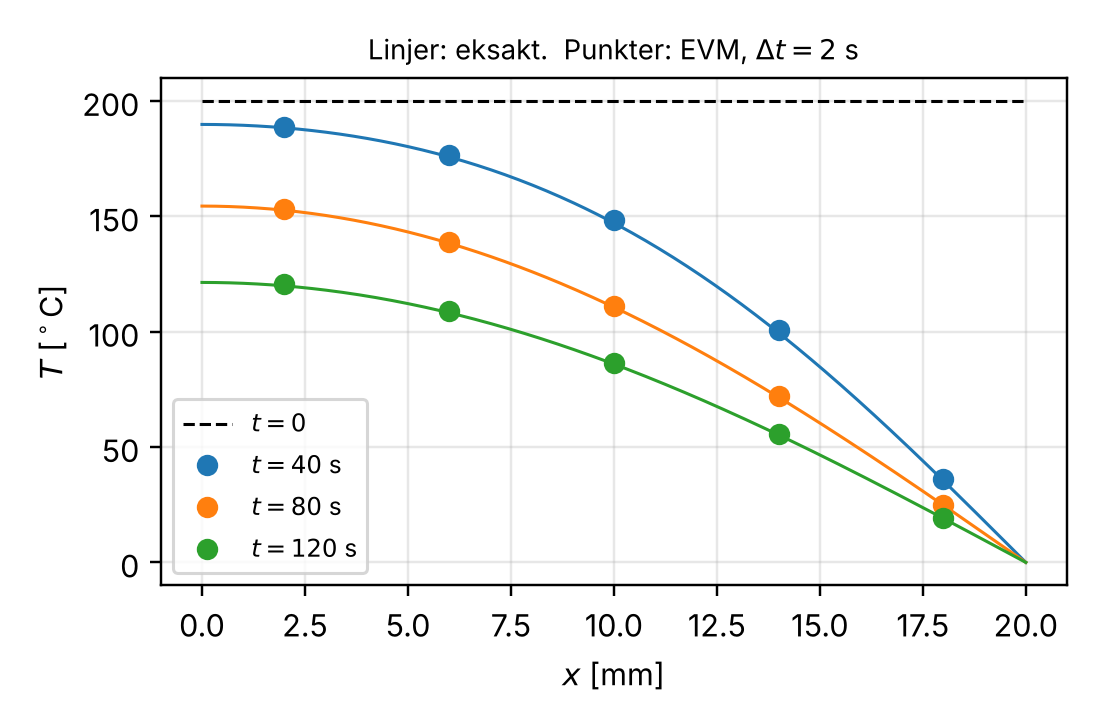
\includegraphics[width=\textwidth]{assets/plate_profiler.png}
\end{column}
\begin{column}{0.46\textwidth}
\scriptsize
\setlength{\tabcolsep}{3pt}
\begin{tabular}{llccccc}
\toprule
$t$ & & 1 & 2 & 3 & 4 & 5 \\
\midrule
40 s & EVM & 188.6 & 176.4 & 148.3 & 100.8 & 35.9 \\
 & eksakt & 188.4 & 175.8 & 147.1 & 99.5 & 35.4 \\
\midrule
80 s & EVM & 153.3 & 139.1 & 111.3 & 72.1 & 25.0 \\
 & eksakt & 152.7 & 138.4 & 110.6 & 71.6 & 24.8 \\
\midrule
120 s & EVM & 120.5 & 108.8 & 86.5 & 55.6 & 19.2 \\
 & eksakt & 119.9 & 108.2 & 86.0 & 55.3 & 19.1 \\
\bottomrule
\end{tabular}
\medskip

\small Den eksakte løsningen er en Fourier-rekke (kompendiet). Fem kontrollvolum er nok til å følge den godt.
\end{column}
\end{columns}
\end{frame}

\begin{frame}{Hva skjer hvis vi bryter kravet?}
\begin{columns}[c]
\begin{column}{0.52\textwidth}
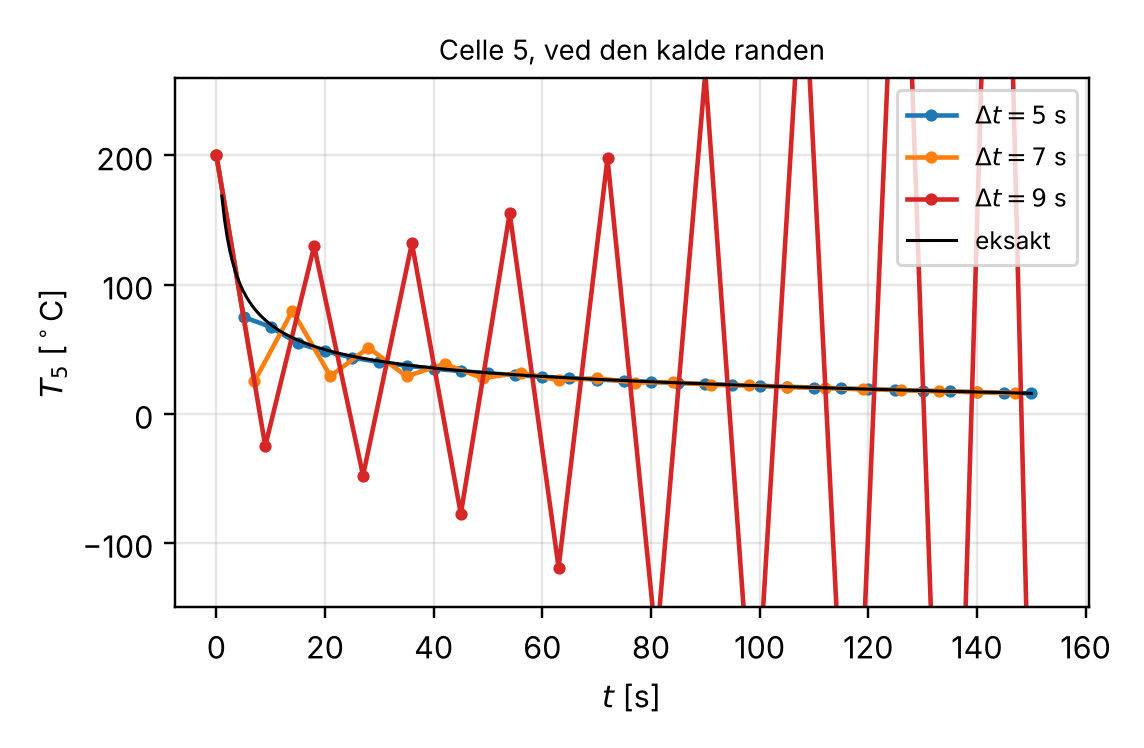
\includegraphics[width=\textwidth]{assets/stabilitet.png}
\end{column}
\begin{column}{0.46\textwidth}
\small
\begin{itemize}
\item \textbf{$\Delta t = 5$ s:} alle krav oppfylt -- fysisk riktig.
\item \textbf{$\Delta t = 7$ s:} bare kravet i \emph{randcellen} er brutt. $T_5$ hopper opp og ned ($25, 80, 29, 51, \ldots$) -- i en plate som bare avkjøles! Svingningene dempes ut, men løsningen er ufysisk i starten.
\item \textbf{$\Delta t = 9$ s:} også kravet i de \emph{indre} cellene er brutt. Sagtannmønsteret vokser -- løsningen eksploderer.
\end{itemize}
\begin{oppsumb}{Regel}
Velg $\Delta t$ ut fra den \emph{strengeste} cellen.
\end{oppsumb}
\end{column}
\end{columns}
\end{frame}

\begin{frame}{Lang tid: tilbake til det stasjonære problemet}
\begin{columns}[c]
\begin{column}{0.48\textwidth}
Når temperaturen slutter å endre seg, er $T^{n+1} = T^n$:
\[
\rho c\,A\,\delta x\,\frac{T^{n+1}-T^n}{\Delta t} = F - L\,T^n
\;\Longrightarrow\;
L\,T = F .
\]
Det er nøyaktig det stasjonære problemet fra F23!
\begin{itemize}
\item Staven fra F23 ($100\,^\circ$C og $500\,^\circ$C i endene) starter på $20\,^\circ$C \ldots
\item \ldots og ender i $140, 220, 300, 380, 460$.
\end{itemize}
\end{column}
\begin{column}{0.50\textwidth}
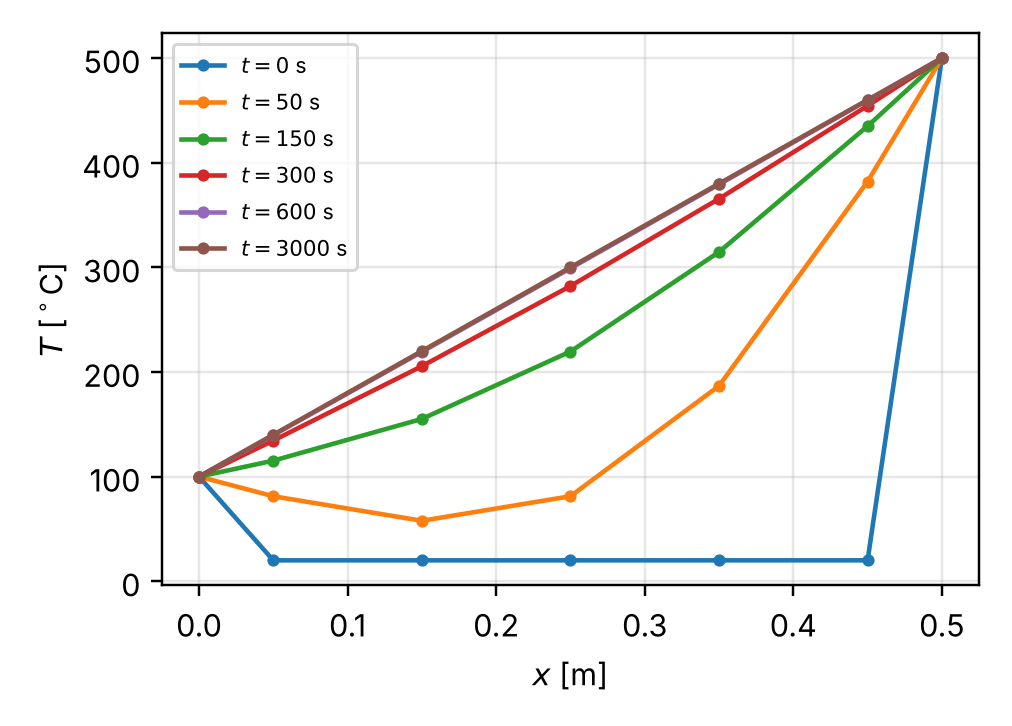
\includegraphics[width=\textwidth]{assets/stav_mot_stasjonaer.png}
\end{column}
\end{columns}
\end{frame}

\section{2D og implisitte skjema}

\begin{frame}{Tidsavhengig i 2D}
\[
T^{n+1} = T^n + \frac{\Delta t}{\rho c\,\delta x\,\delta y\,t}\big(F - L\,T^n\big), \qquad L, F \text{ fra F25.}
\]
\centering
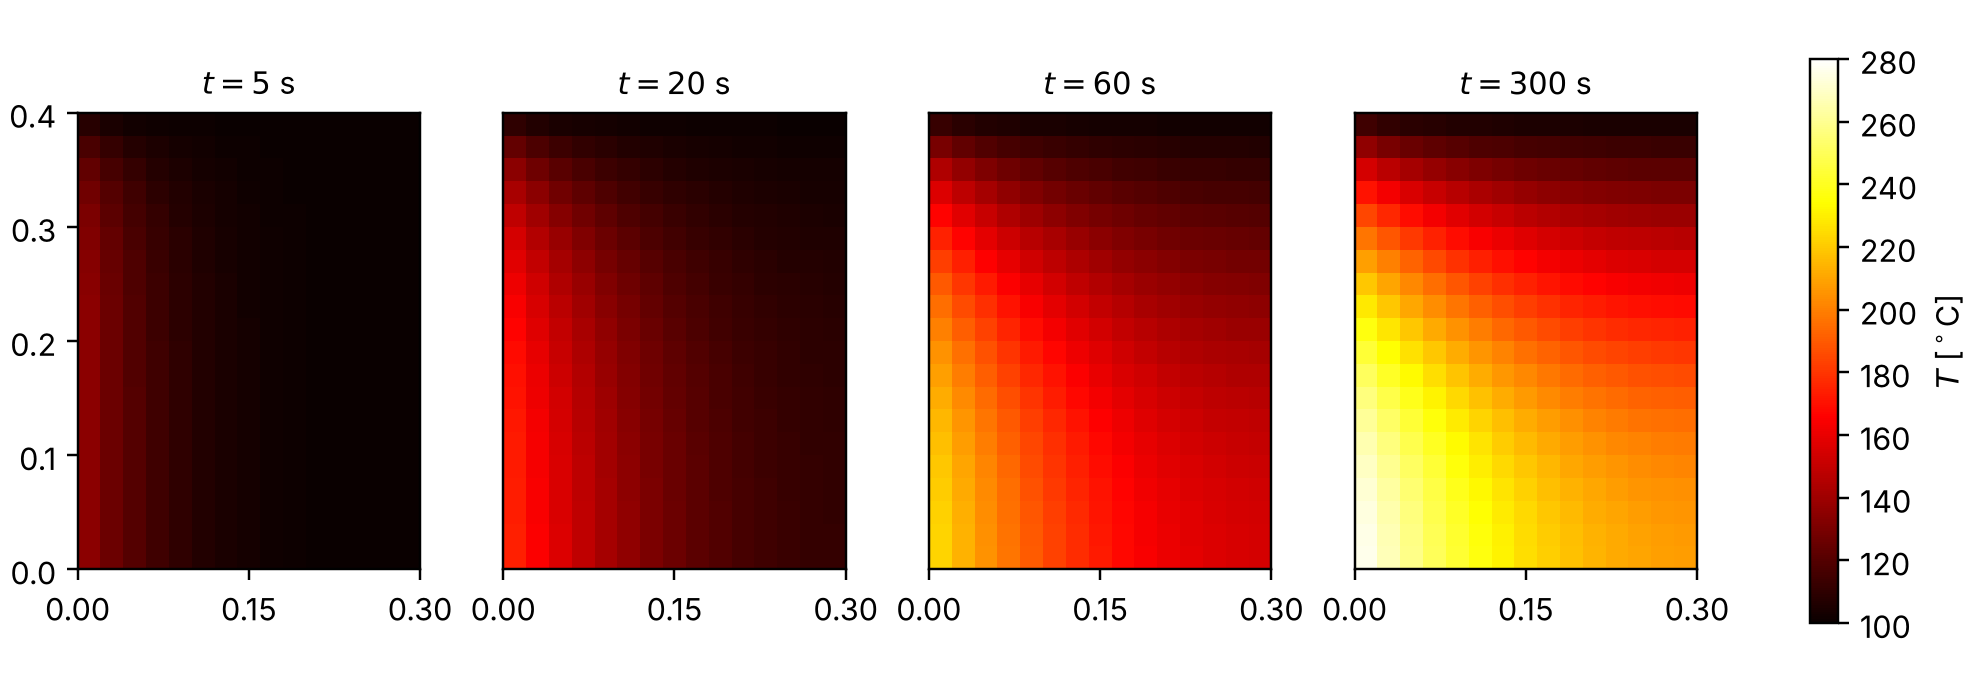
\includegraphics[width=0.78\textwidth]{assets/plate2d_tid.png}
\begin{itemize}
\item Platen fra F25 ($\rho c = 10^6$), startet på $100\,^\circ$C. Varmen trenger inn fra vest.
\item Stabilitet, $\delta x = \delta y = h$: indre $\Delta t \le \rho c\,h^2/(4\kappa)$ ($r\le\frac14$), \; nordveggen $\Delta t \le \rho c\,h^2/(5\kappa)$.
\end{itemize}
\end{frame}

\begin{frame}{Til orientering: implisitte skjema}
Evaluer fluksene ved det \emph{nye} tidsnivået $t_{n+1}$:
\[
\big(a_P^0 + a_W + a_E - S_P\big)\,T_P^{n+1} = a_W\,T_W^{n+1} + a_E\,T_E^{n+1} + a_P^0\,T_P^n + S^u
\]
På matriseform:
\[
\Big(\frac{\rho c\,A\,\delta x}{\Delta t}\,I + L\Big)\,T^{n+1} = \frac{\rho c\,A\,\delta x}{\Delta t}\,T^n + F
\]
\begin{itemize}
\item Alle koeffisienter er positive for \emph{alle} $\Delta t$: \textbf{ubetinget stabilt}.
\item Prisen: et ligningssystem (\texttt{la.solve}) i hvert tidssteg.
\item Stabilt er ikke det samme som nøyaktig: med $\Delta t = 20$ s blir platen ved $t=120$ s ca.\ $5\,^\circ$C for varm.
\end{itemize}
\end{frame}

\section{Oppsummering av kapittel 3}

\begin{frame}{Oppsummering: numeriske metoder for PDE-er}
\begin{columns}[t]
\begin{column}{0.49\textwidth}
\footnotesize
\begin{oppsumb}{Randverdiproblemer}
Laplace, Poisson, stasjonær varmeledning.
\begin{itemize}
\item Ett ligningssystem $L\mathbf u = F$.
\item Randverdiene havner i $F$.
\item Løses direkte (\texttt{la.solve}) eller med Jacobi/Gauss-Seidel.
\end{itemize}
\end{oppsumb}
\begin{oppsumb}{Initialverdiproblemer}
Varmeligningen, bølgeligningen.
\begin{itemize}
\item Marsjer i tid fra initialverdien.
\item Eksplisitte skjema krever lite nok $\Delta t$:\\
varme $r\le\frac12$ (1D), $r\le\frac14$ (2D); \; bølge $c\Delta t/\Delta x\le 1$.
\end{itemize}
\end{oppsumb}
\end{column}
\begin{column}{0.49\textwidth}
\footnotesize
\begin{oppsumb}{Differanser (FD) og endelig volum (EVM)}
\begin{itemize}
\item FD tilnærmer \emph{de deriverte} i punkter.
\item EVM tilnærmer \emph{fluksene} over flatene, ut fra bevaringsloven på integralform.
\item Samme ligninger i det indre på uniformt gitter.
\item EVM: konservativ, kjent fluks på randen er naturlig, tåler ikke-uniforme gitre.
\end{itemize}
\end{oppsumb}
\begin{oppsumb}{Oppskrift for EVM}
Integrer over kontrollvolum, lineære flukser:
\vspace{-1mm}\[
a_P\phi_P = \textstyle\sum a_{nb}\phi_{nb} + S^u,\quad a_P = \sum a_{nb} - S_P,
\]
randbidrag i $S^u$, $S_P$, og $S_P\le0$.
\end{oppsumb}
\end{column}
\end{columns}
\end{frame}

\begin{frame}{Koding: \texttt{F26\_EVM\_Tidsavhengig.ipynb}}
\begin{enumerate}
\item \textbf{Avkjøling av platen:} \texttt{L} og \texttt{F} som i F24, og tidsløkken \texttt{u[:, i+1] = u[:, i] + \ldots} -- sammenlignet med den eksakte løsningen.
\item \textbf{Stabilitet:} \texttt{dt\_maks = rho\_c*A*deltax / np.diag(L)}, og kjøringer med $\Delta t = 5$, $7$ og $9$ s.
\item \textbf{Fra tidsavhengig til stasjonær:} staven fra F23 varmes opp til $140, \ldots, 460$.
\item \textbf{2D:} platen fra F25, med \texttt{evm\_2d}, som varmekart over tid.
\item \textbf{Til orientering:} et implisitt skjema med \texttt{la.solve} i hvert tidssteg.
\end{enumerate}
\begin{remb}{Prøv selv (i notatboken)}
Finere gitter -- hvor lite blir $\Delta t$? \;$\cdot$\; varmekilde i staven \;$\cdot$\; stabilitetsgrensen i 2D.
\end{remb}
\end{frame}

\end{document}
